\def\year{2020}\relax
%File: formatting-instruction.tex
\documentclass[letterpaper]{article} % DO NOT CHANGE THIS
\usepackage{aaai20}  % DO NOT CHANGE THIS
\usepackage{mathtools}
\usepackage{times}  % DO NOT CHANGE THIS
\usepackage{helvet} % DO NOT CHANGE THIS

\usepackage{courier}  % DO NOT CHANGE THIS
\usepackage[hyphens]{url}  % DO NOT CHANGE THIS
\usepackage{graphicx} % DO NOT CHANGE THIS
\urlstyle{rm} % DO NOT CHANGE THIS
\def\UrlFont{\rm}  % DO NOT CHANGE THIS
\usepackage{graphicx}  % DO NOT CHANGE THIS
\usepackage{subcaption}
\frenchspacing  % DO NOT CHANGE THIS
\setlength{\pdfpagewidth}{8.5in}  % DO NOT CHANGE THIS
\setlength{\pdfpageheight}{11in}  % DO NOT CHANGE THIS
%\nocopyright
%PDF Info Is REQUIRED.
% For /Author, add all authors within the parentheses, separated by commas. No accents or commands.
% For /Title, add Title in Mixed Case. No accents or commands. Retain the parentheses.
 \pdfinfo{
/Title (Stability and Chaos in Multi Agent Reinforcement Learning)
/Author (Aamal Hussain, Francesco Belardinelli)
} %Leave this	
% /Title ()
% Put your actual complete title (no codes, scripts, shortcuts, or LaTeX commands) within the parentheses in mixed case
% Leave the space between \Title and the beginning parenthesis alone
% /Author ()
% Put your actual complete list of authors (no codes, scripts, shortcuts, or LaTeX commands) within the parentheses in mixed case. 
% Each author should be only by a comma. If the name contains accents, remove them. If there are any LaTeX commands, 
% remove them. 

% DISALLOWED PACKAGES
% \usepackage{authblk} -- This package is specifically forbidden
% \usepackage{balance} -- This package is specifically forbidden
% \usepackage{caption} -- This package is specifically forbidden
% \usepackage{color (if used in text)
% \usepackage{CJK} -- This package is specifically forbidden
% \usepackage{float} -- This package is specifically forbidden
% \usepackage{flushend} -- This package is specifically forbidden
% \usepackage{fontenc} -- This package is specifically forbidden
% \usepackage{fullpage} -- This package is specifically forbidden
% \usepackage{geometry} -- This package is specifically forbidden
% \usepackage{grffile} -- This package is specifically forbidden
% \usepackage{hyperref} -- This package is specifically forbidden
% \usepackage{navigator} -- This package is specifically forbidden
% (or any other package that embeds links such as navigator or hyperref)
% \indentfirst} -- This package is specifically forbidden
% \layout} -- This package is specifically forbidden
% \multicol} -- This package is specifically forbidden
% \nameref} -- This package is specifically forbidden
% \natbib} -- This package is specifically forbidden -- use the following workaround:
% \usepackage{savetrees} -- This package is specifically forbidden
% \usepackage{setspace} -- This package is specifically forbidden
% \usepackage{stfloats} -- This package is specifically forbidden
% \usepackage{tabu} -- This package is specifically forbidden
% \usepackage{titlesec} -- This package is specifically forbidden
% \usepackage{tocbibind} -- This package is specifically forbidden
% \usepackage{ulem} -- This package is specifically forbidden
% \usepackage{wrapfig} -- This package is specifically forbidden
% DISALLOWED COMMANDS
% \nocopyright -- Your paper will not be published if you use this command
% \addtolength -- This command may not be used
% \balance -- This command may not be used
% \baselinestretch -- Your paper will not be published if you use this command
% \clearpage -- No page breaks of any kind may be used for the final version of your paper
% \columnsep -- This command may not be used
% \newpage -- No page breaks of any kind may be used for the final version of your paper
% \pagebreak -- No page breaks of any kind may be used for the final version of your paperr
% \pagestyle -- This command may not be used
% \tiny -- This is not an acceptable font size.
% \vspace{- -- No negative value may be used in proximity of a caption, figure, table, section, subsection, subsubsection, or reference
% \vskip{- -- No negative value may be used to alter spacing above or below a caption, figure, table, section, subsection, subsubsection, or reference

\setcounter{secnumdepth}{0} %May be changed to 1 or 2 if section numbers are desired.

% The file aaai20.sty is the style file for AAAI Press 
% proceedings, working notes, and technical reports.
%
\setlength\titlebox{2.5in} % If your paper contains an overfull \vbox too high warning at the beginning of the document, use this
% command to correct it. You may not alter the value below 2.5 in
\title{Stability and Chaos in Multi Agent Reinforcement Learning}
%Your title must be in mixed case, not sentence case. 
% That means all verbs (including short verbs like be, is, using,and go), 
% nouns, adverbs, adjectives should be capitalized, including both words in hyphenated terms, while
% articles, conjunctions, and prepositions are lower case unless they
% directly follow a colon or long dash
\author{Aamal Hussain, Francesco Belardinelli\textsuperscript{\rm 1}\thanks{Something to do with the
CDT}\\ % All authors must be in the same font size and format. Use \Large and \textbf to achieve this result when breaking a line
\textsuperscript{\rm 1}Imperial College London\\ %If you have multiple authors and multiple
% affiliations
% use superscripts in text and roman font to identify them. For example, Sunil Issar,\textsuperscript{\rm 2} J. Scott Penberthy\textsuperscript{\rm 3} George Ferguson,\textsuperscript{\rm 4} Hans Guesgen\textsuperscript{\rm 5}. Note that the comma should be placed BEFORE the superscript for optimum readability
Do we give the address? \fb{normally the submission is blind.}\\
publications20@aaai.org % email address must be in roman text type, not monospace or sans serif
}

\input{macros}

 \begin{document}

\maketitle

\begin{abstract}
Working Abstract
\end{abstract}

\section{Introduction}

\subsection{Contribution}

\fb{possibly add research question below.}

In this study, we will be considering the question: under what parameter selections are is a
multi-agent system, which is trained on an iterated game using Q-Learning, likely to converge to an
equilibrium as opposed to complex behaviours? In investigating this question, we will make the
following assumptions:

\begin{enumerate}
    \item There are a finite set of agent, though the length $p$ of the set is arbitrary. 
    \item The agents have a large, but discrete, strategy space: during the theoretical study, we
    will make the assumption that the number of actions $N \rightarrow \infty$.
    \item The agents are homogeneous. This requires that all agents have the same parameters and are
    trained using the same algorithm. Since this is typically the case in reinforcement learning
    studies, it is not an unreasonable assumption, but does present an interesting avenue for future
    work.
    \item The agents are trained on stateless, normal form games (i.e. the environment is static).
\end{enumerate}

The parameters that we will consider are:

\begin{enumerate}
    \item $\alpha \in [0, 1]$: the \em{step length}. Low values of $\alpha$ denote smaller
    updates. Heuristically we can consider this to be the memory of the agent: lower $\alpha$
    denotes longer memory.
    \item $\tau in [0, \infty)$: the \em{intensity of choice}, as termed by Sanders et al. 
    \cite{Sanders2018}. This is sometimes written as $\beta$ in the literature \cite{Sutton2018}.
    $\tau = 0$ results in all actions being selected with equal probability, regardless of their
    Q-value, whilst $\tau \rightarrow \infty$ results in the action with the highest Q-value chosen
    at every step. This may be considered the \em{exploration-exploitation parameter}. For greater
    details into these parameters, the interested reader should consult \cite{Sutton2018}.
    \item $\Gamma \in [-1, p-1]$: the \em{payoff correlation}. This term controls the choice of
    covariance matrix from which random payoff matrices are drawn. $\Gamma = -1$ indicates a zero
    sum game, in which the sum of payoffs for a given action across all agents is 0, resulting in a
    purely competitive game. $\Gamma = p-1$ gives a purely co=operative game in which all agents
    share the same payoffs. The manner in which a game is generated from the choice of $\Gamma$ is
    described in Section \ref{sec::Theory} and follows the same procedure as outlined in \cite{Sanders2018}.
\end{enumerate}

\subsection{Related Work}

\fb{feel free to add the Related Work}

\section{Preliminaries}

In this section we will establish some of the preliminaries which are
required to follow the subsequent sections. The first is \em{Dynamical Behaviours} \fb{maybe italics?} 
which considers the evolution of agent strategies as they
learn on an iterated game. This study aims to classify, based on the
agent parameters and the payoff matrices, which of these behaviours
will be seen. The second is \em{Dynamics of Q-Learning}. These are a set
of equations which model the aforementioned strategy evolution. It is
on these dynamics that we will perform our analysis.

\subsection{Dynamical Behaviours}

 This segment of research aims to achieve a deeper understanding
    of the strategy evolution of agents following a Q-Learning
    approach. This allows for guarantees to be placed on the behaviour
    of such agents, in particular the conditions under which the game
    will converge to a stable equilibrium.

    It has long been established that, upon lifting the strong
    assumptions made by traditional game theory (such as the
    rationality of agents and complete information), player
    strategies can result in much more complex behaviour than
    convergence to a Nash Equilibrium (NE). In fact, this is even true
    on what would commonly be regarded as 'simple' games such as
    tic-tac-toe and prisoner's dilemma \cite{Galla2011,
      Sato2002}. These behaviours include: convergence to a unique
    equilibrium (though not always to an NE), convergence to one of
    multiple equilibria, limit cycles and chaos. These behaviours are
    shown in Figure \ref{fig::DynamicalBehaviours}. Of these, the most
    preferable is, of course, convergence to a unique equilibrium,
    although it is still possible to study systems with multiple
    equilibria or limit cycles \cite{Strogatz2000}. However, it would
    be difficult to control systems whose dynamics are governed by
    chaos (though research into controlling chaos is ongoing and rife
    with opportunity \cite{Fradkov2009}) and so MARL techniques should
    avoid this. It would, therefore, be a useful endeavour to
    determine the conditions under which these sorts of behaviours
    arise.

    \begin{figure}[h]
        \centering
        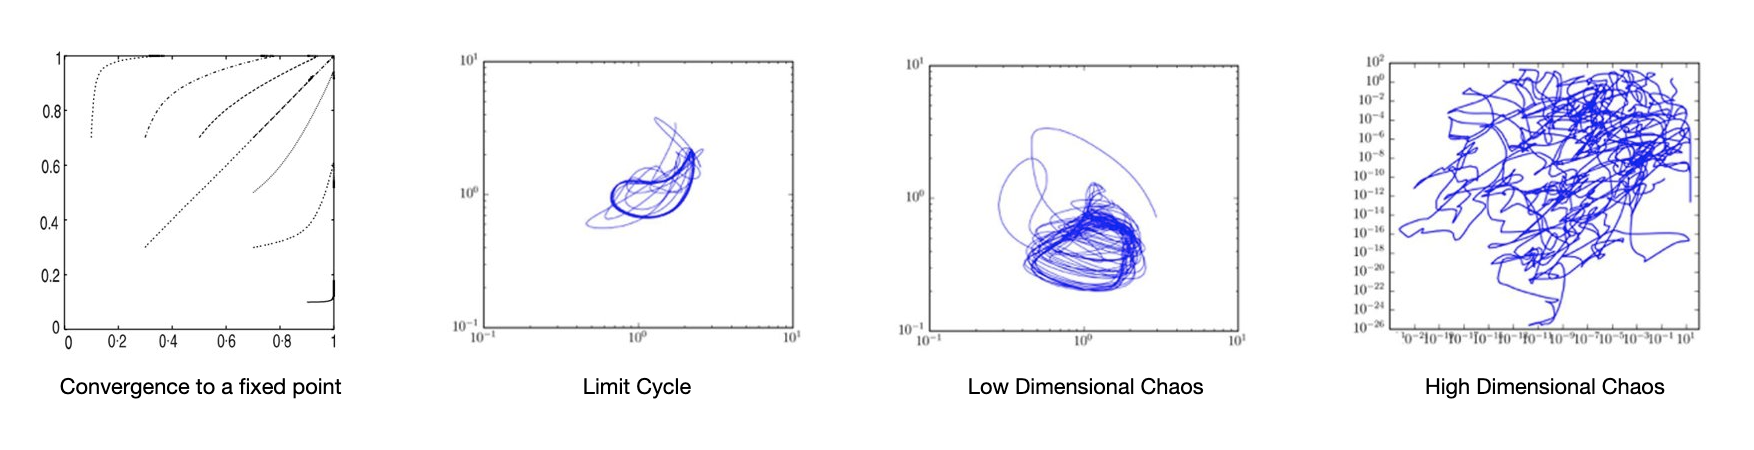
\includegraphics[width=1.1\textwidth]{Figures/DynamicalBehaviours}
        \caption{ \label{fig::DynamicalBehaviours} Different types of dynamical behaviour
       displayed
        by learning agents. Here the x-axis is the probability with which agent 1 chooses a given action, whilst the y-axis denotes the same probability for agent 2. a) Figure drawn from \cite{Tuyls2006AnGames}.
        Convergence
        to a unique fixed point in the upper right corner (1, 1). This fixed point is unique, in
        that all trajectories, regardless of initialisation, will converge to this point. b) Limit Cycle, the trajectories converge to cyclic behaviour c,
        d) Chaotic behaviour, here small deviatons in the initial conditions can grow
        exponentially. b-d drawn from \cite{Sanders2018}}
\fb{one figure from a reference is fine, but two maybe are not necessary.}
    \end{figure}

\subsection{Dynamics of Q-Learning}

The behaviour of a system may be studied given a model of its
    dynamics. It is through this process that a wide array of physical
    systems, from harmonic pendulums to geophysical fluids, can be
    understood. A growing body of research aims to understand
    multi-agent reinforcement learning through the lens of its
    dynamics. In this light, Tuyls et al. \cite{Tuyls2006AnGames} were able to derive a continuous time dynamical
system describing how agents following a Q-Learning approach adjust the probabilities of choosing actions
as they iteratively play a game.  Through this, they were able to
    arrive at the following model of Multi-Agent Q-Learning

    \begin{subequations}
    \label{eqn::EOM}
        \begin{equation}
            \frac{\dot{x}(t)}{x(t)} = \alpha \tau (\sum_{j} a_{ij} y_j - \sum_{i j} x_i a_{ij} y_j)
            + \alpha \sum_j x_j ln(\frac{x_j}{x_i}) 
        \end{equation}
        \begin{equation}
            \frac{\dot{y}(t)}{y(t)} = \alpha \tau (\sum_{j} b_{ij} x_j - \sum_{i j} y_i b_{ij} x_j)
            + \alpha \sum_j y_j ln(\frac{y_j}{y_i}).
        \end{equation}
    \end{subequations}

    Here, $\alpha$ and $\tau$ are the parameters of the agent; Sanders et al. refer to these as the
    memory and intensity of choice parameters respectively \fb{what are $\alpha$ and $\tau$ exactly?}. Agent 1 takes action $i$ with probability
    $x_i$ while Agent 2 takes action $j$ with probability $y_j$. If these actions are taken, the agents
    receive payoff $a_{ij}$ and $b_{ji}$ respectively. With these equations, it is possible to
    predict the expected behaviour of Q-Learning agents, as shown in Figure 
    \ref{fig::TuylsExperiments}. Upon examination of the derivation in \cite{Tuyls2006AnGames}, it
    is clear that the dynamics generated give the expected behaviour and, therefore , cannot account
    for transients. It is also interesting to note that the dynamics (\ref{eqn::EOM}) do not include
    the parameter $\gamma$, which moderates the Q-update. The implication is that this has no effect
    on the expected behaviour of the system. \textbf{Shall I include some tests to confirm this?
    It does turn out to be mostly true, the value of $\gamma$ doesn't affect the overall behaviour,
    but rather results in smaller or larger steps. What do you think?}.
    as well}.

    \begin{figure}
    \centering
        \begin{subfigure}[b]{0.9 \textwidth}
            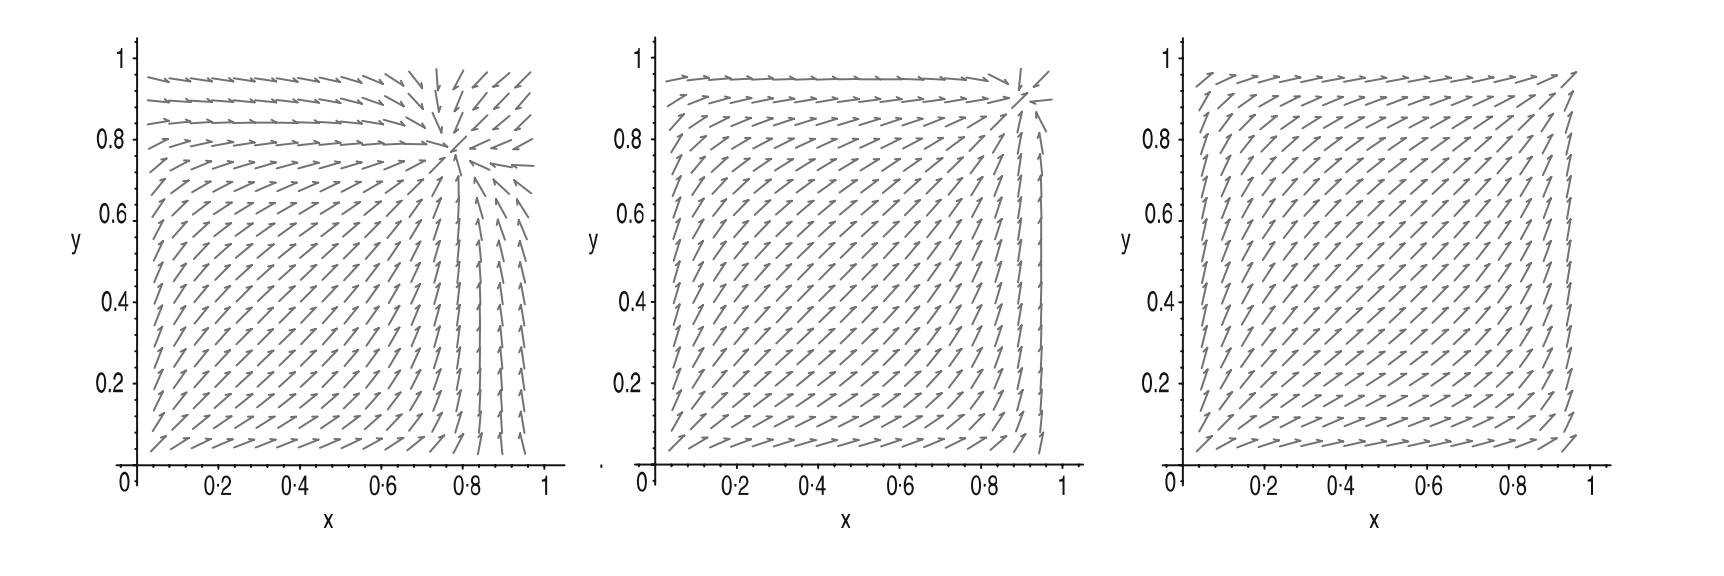
\includegraphics[width=0.52 \textwidth]{Figures/Dynamics}
            \caption{}
        \end{subfigure}
        
        \begin{subfigure}[b]{0.9 \textwidth}
            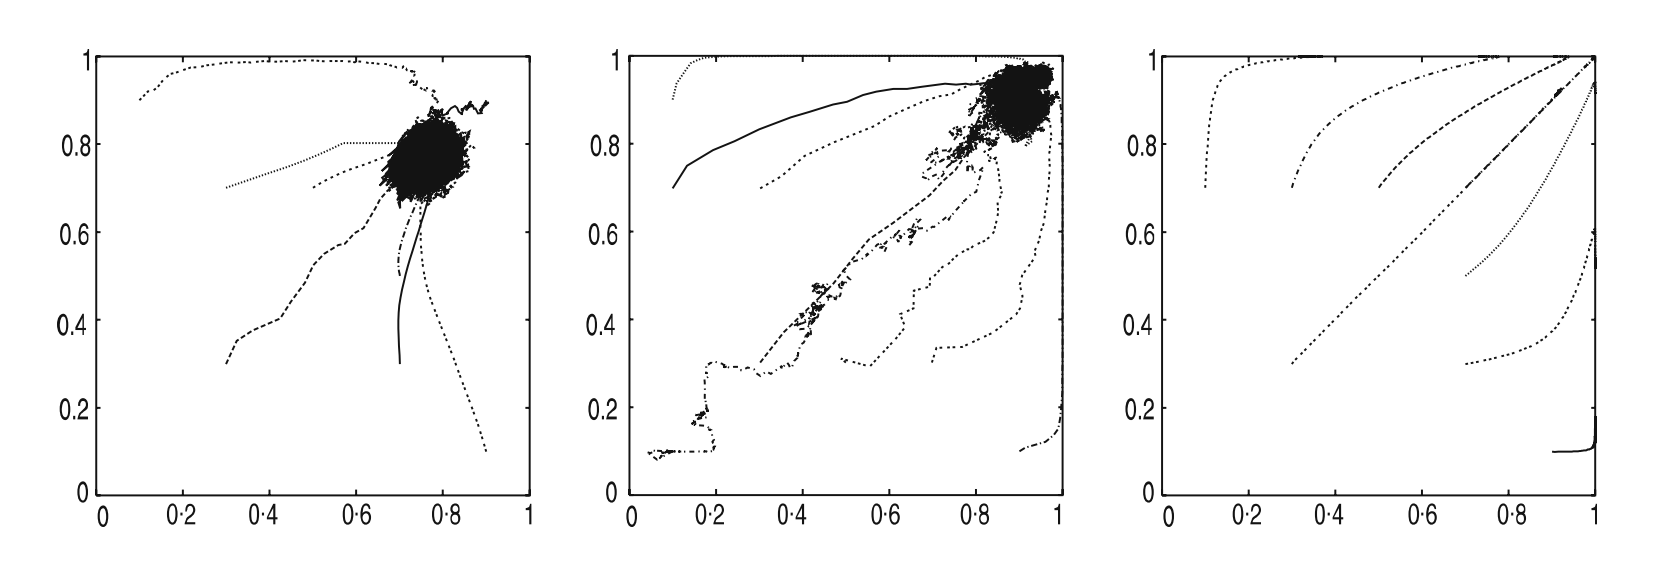
\includegraphics[width=0.5 \textwidth]{Figures/Q-Learners}
            \caption{}
        \end{subfigure}

        \caption{ \label{fig::TuylsExperiments} Figures taken from \cite{Tuyls2006AnGames} a) Phase
        plot showing the expected behaviour of Q-Learning agents trained by iterating the
        Prisoner's Dilemma game as predicted by (\ref{eqn::EOM}). From left to right, the agents
        have parameter $\tau = 1, 2, 10$. b) Corresponding trajectories of Q-Learning agents with
        randomised initial conditions displayed through numerical simulation. It is clear that the
        trajectories in b) follow the predictions in a), if transients are neglected. }
    \end{figure}    

    It is clear, both from (\ref{eqn::EOM}) and Figure \ref{fig::TuylsExperiments}, that the long-term strategy selection of
    these agents is determined by the parameters $\alpha, \tau$ and the payoffs $a_{ij}, b_{ij}$. We
    then pose the question: how do these elements influence the types of behaviours seen during
    learning on an iterated game? In other words, under what parameter selections are we likely to
    see convergence to unique equilibria, multiple equilibria, limit cycles or chaos? \fb{state this explicitly as a research question, possibly in the contribution.}

\section{Determination of Phase Transition Line} \label{sec::Theory}

\fb{what will be the content of this section? is it the derivations?}

\section{Experimental Evaluation}

To verify our theoretical results, and to examine the underlying structure of stability and chaos in
Multi-Agent Q Learning, we perform a series of numerical experiments by varying the parameters $\Gamma$ and
$\alpha$ whilst keeping $\tau$ fixed. The purpose of this experiment was to determine a heuristic estimate for the Lyapunov exponent, which determines whether initial conditions which start close to one another will converge or diverge from each other. The former indicates a stable system (in the sense of Lyapunov) whilst the latter signals instability \cite{Strogatz2000}.

This yields the result shown in
Figure \ref{fig::NumericalExperiments}. We see from this that the stability of the system is highly dependent on
the value of $\tau$.
For
low values, the system converges almost everywhere, whilst increasing $\tau$ to 0.15 decreases
the probability of convergence significantly.

\begin{figure}[h]
    \centering
     \begin{subfigure}[b]{0.45 \textwidth}
    \centering
    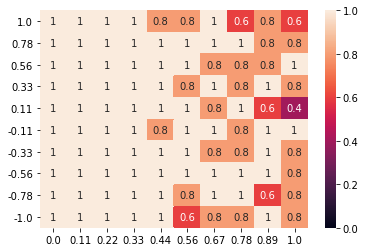
\includegraphics[width = 0.7 \textwidth]{Figures/AlphaRun_tau_005.png}
    \caption{$\tau = 0.05$}
    \end{subfigure}
    \begin{subfigure}[b]{0.45 \textwidth}
    \centering
    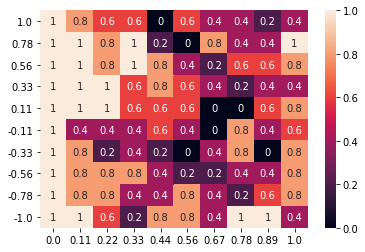
\includegraphics[width = 0.7 \textwidth]{Figures/tau_015.png}
    \caption{$\tau = 0.15$}
    \end{subfigure}

    \caption{$\tau = 0.05$, $\gamma = 0.75$, $\alpha \in [0, 1]$, $\Gamma \in [-1, 1]$. Each
    simulation is run for 1 $\times 10^4$ iterations and the Lyapunov exponent is determined. For each
    combination of $\alpha$, $\Gamma$ the game is played 100 times, each with random payoff matrices
    and initial conditions. The average Lyapunov exponent is determined and shown in the heatmap.
    \label{fig::NumericalExperiments}}
\end{figure}

   To generate the numerical simulations in Figure \ref{fig::NumericalExperiments} we used the
   following procedure.

   \begin{enumerate}
   	\item Fix the paremeters $\tau, \gamma$. The latter is held at 0.75 in all experiments as (\ref{eqn::EOM}) indicates that the value of $\gamma$ does not affect the overall behaviour of the system.
   	\item Initialise values of $\Gamma, \alpha$. These will be swept over in the experiment.
	\item Generate payoff matrices for both agents by sampling from a multi-variate Gaussian 
    (variables are the payoff elements) with mean zero and covariance parameterised by $\Gamma$. \textbf{Put these in the derivation}.
    \item Initialise 2 sets of agents (denote their action probabilities as $\Vec{A_1}$ and $\Vec{A_2}$ respectively) each with random initial conditions (i.e. random action probabilities).
    \item Allow both sets of agents to learn over a maximum of $1 \times 10^4$ iterations.
    \item After 300 iterations measure the distance $\Vec{\delta_1} = |A_2 - A_1|$
    \item After 10000 iterations measure the distance $\Vec{\delta_n} = |A_2 - A_1|$
    \item Determine 

    \begin{equation}
        \lambda_n = \max_{i} 10^{-4} ln(\delta_{n, i}/\delta_{1, i})
    \end{equation}

   \end{enumerate}

\fb{Liapunov $\to$ Lyapunov}

\section{Conclusion}

\subsection{Future Work}


\bibliography{references}
\bibliographystyle{aaai}
\end{document}
